\chapter{Design}
\label{ch:Design}

\section{Theoretische Grundlagen}

Zunächst sollen die grundlegenden Eigenschaften der erwarteten Eingangssignale definiert und näher beschrieben werden. 

\subsection{Zeit- und wertdiskrete digitale Signale}

Bei den Eingangssignalen des Event-Recorders handelt es sich um die Ausgänge von Mikrocontrollern oder anderer digitaler Schaltungen und damit um digitale Signal.
Digitale Signale sind durch zwei grundlegende Eigenschaften charakterisiert, sie sind:
\begin{itemize}
	\item \textbf{zeitdiskret}, und
	\item \textbf{wertdiskret}
\end{itemize}
\textbf{Wertdiskret} bedeutet, dass das Signal nur genau einen Wert aus einer festgelegten Anzahl möglicher Werte-Zustände annehmen kann.
In den meisten Fällen beschränkt sich der Wertebereich auf die Binärwerte ``1'' oder ``0'', das heißt ein digitales Signal ist zum Beispiel bei 0,1 Volt Spannung ``0'' und bei 3,2 Volt ``1'', wohingegen ein analoges Signal alle möglichen Werte zwischen 0 und 3,3 Volt annehmen kann.\\

\textbf{Zeitdiskret} bedeutet, dass ein digitales Signal ``nur zu bestimmten periodischen Zeitpunkten definiert ist beziehungsweise nur dann eine Veränderung im Signalwert aufweist''\cite{wiki:Digitalsignal}, das heißt dass das Signal bei der Erfassung mit einem festen ``Zeitraster'' abgetastet wird und zwischen den Rasterpunkten einen festen Wert behält.

Bei der Erfassung digitaler Signale ist es nötig, dass die Abtastfrequenz nach Nyquist-Shannon-Abtasttheorem mindestens doppelt so hoch als die maximale Frequenz des untersuchten Signals sein muss, damit das Ausgangssignal ohne Informationsverlust abgebildet werden kann (vgl. \cite{wiki:Digitalsignal}).

Es ist zu beachten, dass es sich bei der Definition von digitalen Signalen um eine idealisierte Ansicht handelt und dass sich bei realen digitalen Signale oft -- vor allem bei hohen Frequenzen -- Störeffekte zeigen. Ein Beispiel für einen Störeffekt wäre das ``Prellen'' eines mechanischen Schalters, bei dem es durch den mechanischen Kontakt zu einem mehrfachen Signalwechsel kommen kann, bevor ein stabiles Signal anliegt. Wenn der Schalter-Zustand dabei mit vergleichsweise langsamer Geschwindigkeit ausgelesen wird, gehen die deutlich schnelleren Signalwechsel gemäß dem Nyquist-Shannon-Abstasttheorem nicht in das Ausgangssignal ein, bei entsprechend hoher Abtastrate werden sie allerdings mit in Ausgangssignal übernommen und können dann unerwünschte Effekte auslösen.\\
Bei der in dieser Arbeit verwendeten Hardware sind keine speziellen Vorrichtungen vorhanden um solchen Effekten entgegen zu wirken, das heißt es wird am Eingang ein für die Analyse ausreichend stabiles Signal erwartet.   \\

Damit die Ergebnisse des Event-Recorders richtig auswertet werden können, muss zu jeder Signaländerung der ``diskrete'' Zeitpunkt bekannt sein, das heißt das Zeitraster der Abtastung muss numeriert werden, so dass jeder Signaländerung ein eindeutiger Zeitstempel zugeordnet werden kann.
Diese ``Numerierung'' wird umgesetzt, in dem der von einem Oszillator\footnote{Eigener Hardware-Baustein, der eine konstant auf- und abschwingende Spannung erzeugt und damit zur Taktung digitaler Schaltung verwendet werden kann} generierte Schaltungstakt mit einer Zählerschaltung aufaddiert wird. Der Zeitstempel entspricht dann einfach dem aktuellen Zählerstand.\\


\begin{table}[h]
\centering
\begin{tabular}{|l|l|l|}
\hline
\rowcolor[HTML]{EFEFEF} 
	EVENT\_ID [8 Bit] & INPUT\_DATA [8 Bit] & TIMESTAMP [16 Bit]\\ \hline
	\multicolumn{1}{|c|}{0x02} & \multicolumn{1}{c|}{0x01} & \multicolumn{1}{c|}{0x0EF8} \\ \hline
\end{tabular}
\caption{Beispielhafte Darstellung eines aufgenommenen Events mit 16-Bit Zeitstempel}
\label{my-label}
\end{table}


Die Bit-Breite des Zählers legt zusammen mit der Geschwindigkeit des Takts die maximal mögliche Aufnahmelänge fest. Der in dieser Arbeit verwendete Zähler hat eine Breite von 46 Bit, womit sich bei einer Taktfrequenz von 100 Mhz zum Beispiel eine Laufzeit von ca. 195 Stunden ergibt\footnote{Berechnung: \(2^{46} * \frac{1}{100 Mhz} = 2^{46} * 10 ns =\) 195 Stunden, 28 Minuten und 7,422 Sekunden} (was für die meisten Anwendungsfälle mehr als ausreichend ist). 



\subsection{Definition ``Event''}

Für diese Arbeit soll unter dem Begriff ``Event'' ein vom Benutzer festgelegter Signalzustand oder eine Signaländerung an den Eingangspins des Event-Recorders verstanden werden. In den meisten Fällen macht es mehr Sinn eine Signaländerung zu definieren, als einen Zustand, da bei einem anhaltenden Zustand auch das Event kontinuierlich ``ausgelöst'' wird, und ein dementsprechend hohes Datenvolumen erzeugt.\\
Es ergeben sich folgende Definitionsmöglichkeiten für die einzelnen Eingangs-Pins:
\begin{itemize}
	\item ``0'': niedriger logischer Pegel
	\item ``1'': hoher logischer Pegel
	\item ``u'': steigender Pegel
	\item ``d'': fallender Pegel
	\item ``x'': beliebiger Zustand ("don't care") 
\end{itemize}
Zusätzlich wäre eine Kombination von ``u'' und ``d'' denkbar, die auf beliebige Signaländerungen reagiert.
Eine Verkettung dieser Möglichkeiten bei der jedem Eingangspins ein Zustand zugewiesen wird soll als ``Event-Trigger'' -- also als Auslöser eines bestimmten Events -- bezeichnet werden.\\
Dies entspricht im Wesentlichen der Definition von \textit{Trigger} die bei ``traditionellen'' Logikanalysatoren verwendet wird, allerdings mit dem Unterschied dass der Trigger bei einem ``traditionellen'' Logikanalysator die eigentliche Aufnahme einmalig auslöst, und dann bis zum Ende der Aufnahme nicht mehr von Bedeutung ist, während ein Event-Trigger als Teil der Aufnahme kontinuierlich überprüft werden muss und erst bei Erfüllung der Trigger-Bedingung überhaupt Ausgangsdaten generiert werden.\\
Es bietet sich an einem Event zusätzlich bestimme Funktionen zuweisen zu können, wie zum Beispiel das Starten\footnote{Die Erkennung eines Start-Events erfordert folglich, dass auch im ``Ruhezustand'' eine Event-Erkennung durchgeführt wird} und Stoppen der Event-Erkennung, oder das Wechseln in einen zusätzlichen Modus, bei dem alle Signaländerungen ein Ausgangs-Event produzieren (``Dump''-Modus).\\
Wie in der Einführung erwähnt soll die Definition der Events in Text-Form möglich sein und kann dann zum Beispiel für 8 Eingangspins folgendermaßen aussehen:

\begin{lstlisting}[language=yaml]
# event configuration
events: 
  - start:
          trigger: uxxxxxxx
          function: start

  - stop:
          trigger: dxxxxxxx
          function: stop

  - event1:
          trigger: 1uxxxxxx

  - event2:
          trigger: 1xuxxxxx
          function: dump_begin
...
\end{lstlisting}

\clearpage
\section{Überblick der benötigten Hard- und Software-Komponenten}
\subsection{Datenerfassung: FPGA}
Wie im vorherigen Kapitel beschrieben wird für die Datenerfassung eine Zählerschaltung benötigt, die einen stabilen Zeitstempel liefern kann. Voraussetzung dafür ist, dass der Zähler kontinuierlich läuft und nicht durch andere Vorgänge unterbrochen werden kann. Dies ist bei PC-Systemen oder auch Mikrocontrollern nicht ohne weiteres möglich, da die Programmausführung zu jedem Zeitpunkt von Betriebssystem-Funktionen oder Interrupt-Routinen\footnote{Bei einer Interrupt-Routine wird die aktuelle Programmausführung auf CPU-Ebene pausiert, zum Beispiel um auf Ereignisse externer Hardwaregeräte reagieren zu können} pausiert werden kann.\\
Deswegen bietet sich hier die Verwendung einer programmierbaren logischen Schaltung wie zum Beispiel eines CPLDs (\acrlong{CPLD}) oder FPGAs (\acrlong{FPGA}) an, bei dem eine von anderen Komponenten zeitlich vollkommen unabhängige parallele Ausführung des Zählers möglich ist.\\
Sowohl CPLD- als auch FPGA-Chips bestehen aus einer Vielzahl von einheitlichen Blöcken die einfache logische Funktionen abbilden können (in der folgenden Abbildung ``PLBs'', also ``Programmable Logic Blocks'' bezeichnet). Im Vergleich zu logischen Gattern sind die die Blöcke in ihrer Funktion aber frei konfigurierbar. Durch die Vernetzung der so konfigurierten Blöcke können umfangreiche digitale Schaltungen realisiert werden.\\
FPGAs sind etwas komplexer aufgebaut als CPLDs, dabei aber auch flexibler bei der Vernetzung und enthalten oft zusätzliche Funktionsblöcke wie den in der nachfolgenden Abbildung erkennbaren Block-RAM als Zwischenspeicher für größere Datenmengen oder die \acrshort{PLL}-Einheit zur Erzeugung von Taktsignalen mit konfigurierbarer Geschwindigkeit (vgl. \cite{wiki:PLD}).

\begin{figure}[htbp]
	\centering
		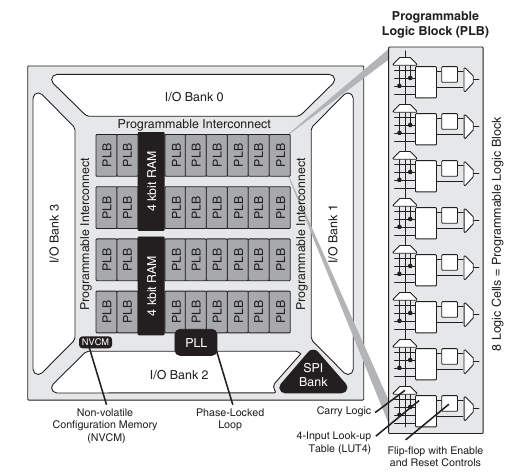
\includegraphics[width=0.80\textwidth]{../figures/iCE40_block_diagram.png}
	\caption[Blockdiagramm des verwendeten iCE40 FPGAs]{Aufbau des verwendeten iCE40 FPGAs (Quelle: iCE40 Datasheet{\cite{doc:datasheet}})}
	\label{fig:ice40_block_diagram}
\end{figure}

Zusätzlich ist die Anzahl von Funktionsblöcken bei FPGAs üblicherweise deutlich höher als als bei CPLDs, weswegen in dieser Arbeit ein FPGA-Chip verwendet werden soll.

Die in der Abbildung erkennbaren I/O-Bänke beinhalten GPIO-Pins die als Ein- oder Ausgänge konfiguriert und direkt mit den Logikblöcken (``PLBs'') im FPGA verbunden werden können.

\subsection{Datenzwischenspeicher: SRAM}

Nach der Erfassung müssen die Daten zwischengespeichert werden. Dabei sind vor allem zwei Faktoren entscheidend:
\begin{itemize} 
	\item Die \textbf{Geschwindigkeit} des Speichers, die meist den maximalen Datendurchsatz der Gesamtschaltung bestimmt
	\item Die \textbf{Größe} des Speichers, die festlegt wie lange bei hohem Datendurchsatz aufgenommen werden kann 
\end{itemize}
Die meisten nicht-flüchtigen Speicher sind aufgrund der unzureichenden Lese- und Schreib-Geschwindigkeiten nicht für diesen Verwendungszweck geeignet, weswegen sich die Verwendung von \acrshort{RAM}-Speicher anbietet. \\
Bei Mikrocontrollern und kleineren FPGA-Boards werden aus Kostengründen und wegen der unkomplizierten Ansteuerung oft SRAM-Speichereinheiten verbaut. SRAM-Speicher hat meist sehr kurze Zugriffszeiten, allerdings bei einer geringen Speichergröße von wenigen MBit. Der in dieser Arbeit verwendete SRAM-Speicher hat beispielsweise eine Größe von 4 Mbit (512 KB) und könnte damit maximal 62500 Events zwischenspeichern\footnote{Bei einer angenommenen Event-Größe von 64-Bit, und unter der Annahme dass der SRAM-Speicher ausschließlich zum Zwischenspeichern von Events verwendet wird}.\\
Bei kontinuierlicher Erfassung von Eingangssignalen mit einer Abtastrate von 100 Mhz entspricht dies einer Aufnahmezeit von unter einer Millisekunde\footnote{$62500 * 10 ns = 0.625 ms$}. Da allerdings keine Eingangssignale erwartet werden, bei denen Events mit einer Frequenz von 100 Mhz auftreten und außerdem bereits bei laufender Aufnahme Events aus dem RAM-Speicher entnommen und weiter übertragen werden, kann der SRAM-Speicher trotzdem im Sinne der Aufgabenstellung als Zwischenspeicher verwendet werden.\\
Als Alternative könnte DRAM-Speicher verwendet werden, der ein Vielfaches der Speicherkapazität bietet und damit auch längere Aufnahmen bei hoher Signaldichte ermöglichen würde. DRAM-Speicher erfordert allerdings im Vergleich zu SRAM ein kontinuierliches ``Auffrischen'' der Speicher-Inhalte durch eine Controller-Einheit und bedeutet dementsprechend deutlich mehr Aufwand und hohe Timinganforderungen bei der Implementierung.


\subsection{Datenübertragung: SPI}

Nach der Datenerfassung und Zwischenspeicherung werden die Daten an ein externes System übertragen, an dem sie weiterverarbeitet oder ausgewertet werden können. Zur Datenübertragung gibt es eine Vielzahl von Schnittstellen und Protokollen. Dabei werden die Daten im Normalfall ``serialisiert'', das heißt wenn ein Event aus 64 Bits besteht, werden die Bits nacheinander über eine einzige Datenleitung übertragen. Geläufige serielle Datenübertragungsverfahren sind vor allem \acrshort{UART}, \acrshort{I2C} und \acrshort{SPI}.
\begin{description}
	\item Bei einem \textbf{UART (\acrlong{UART})} werden die Daten über eine Empfangs- und eine Sendeleitung ausgetauscht. Es wird kein eigenes Taktsignal übertragen, weswegen auf beiden Seiten eine feste Übertragungsgeschwindigkeit (``Baud-Rate'') eingestellt werden muss. UART-Schnittstellen sind weit verbreitet und verhältnismäßig einfach zu implementieren, dabei allerdings recht fehleranfällig und bei üblichen Baud-Raten ist die Übertragungsgeschwindigkeit stark limitiert (vgl. \cite{wiki:UART}).
	\item \textbf{\acrshort{I2C} (\acrlong{I2C})} ist ein synchroner Datenbus, bei dem eine eigene Leitung für den Takt und eine Datenleitung verwendet wird. $\text{I}^2$C arbeitet nach dem Master-Slave-Prinzip, das heißt es können auch mehrere Geräte miteinander kommunizieren. $\text{I}^2$C untertützt Übertragungsraten bis zu 5 Mbit/s (unidirektional, vgl. \cite{wiki:I2C}).
	\item \textbf{\acrshort{SPI} (\acrlong{SPI})} ist wie $\text{I}^2$C ein synchroner Datenbus nach dem Master-Slave-Prinzip. Neben der Leitung für den Takt wird eine Daten-Leitung in Senderichtung und eine Datenleitung in Empfangsrichtung verwendet. Zusätzlich wird pro Gerät eine ``Chip-Select'' Leitung benötigt, um die Geräte adressieren zu können. SPI kann Übertragungsraten bis in den mehrstelligen Megabit-Bereich ermöglichen (vgl. \cite{wiki:SPI}).
\end{description}

Aufgrund der hohen Übertragungsrate und der relativ unkomplizierten Implementierungsmöglichkeiten soll SPI für die Datenübertragung verwendet werden.


\subsection{Steuerung der Aufnahme und sequentielle Programmabläufe}

Neben der reinen Datenerfassung und -Übertragung werden noch Komponenten zur Steuerung und zur Kontrolle des Aufnahmevorgangs benötigt.\\
Grundsätzlich können die benötigten Vorgänge- und Zustände (zum Beispiel das Starten und Stoppen der Aufnahme) direkt im FPGA umgesetzt werden. Als Kommunikationsweg zur Steuerung und Konfiguration kann dann wiederum SPI verwendet werden.\\
Bei längeren oder komplexeren Programmabläufen die keine zeitkritische Ausführung erfordern bietet sich die Verwendung eines zusätzlichen Mikrocontrollers an. Da die meisten PC-Systeme keine programmierbaren \acrshort{GPIO}-Pins als SPI-Schnittstelle zur Verfügung stellen, kann ein Mikrocontroller außerdem als Brücke zwischen FPGA und Anwendersystem fungieren, und zum Beispiel die vom FPGA erfassten Daten über einen USB-Port zur Verfügung stellen.\\
Davon abgesehen wird unter Umständen noch zusätzliche Hardware- und Software-Infrastruktur benötigt um das FPGA und den Mikrocontroller zu programmieren und zu konfigurieren.
\clearpage

\section{Auswahl der Software-Toolchain: IceStorm}

Im Normalfall werden FPGAs mit den vom Hersteller angebotenen -- kommerziellen -- Software-Tools programmiert. Da der Quelltext dieser Tools nicht öffentlich zugänglich ist und FPGA-Hersteller keine relevanten Informationen zur Hardwarestruktur von FPGA-Chips veröffentlichen war es für Opensource-Tools bisher nicht möglich eine Alternative zu den kommerziellen Toolchains der Hersteller zu bieten.\\
Mit der IceStorm-Toolchain wurde erstmals die Hardwarestruktur der -- relativ einfach aufgebauten -- Lattice iCE40 Produkt-Serie\footnote{Es werden nicht alle Chips der iCE40-Serie unterstützt, die verwendbaren Produktvarianten sind auf der IceStorm-Website aufgelistet\cite{web:IceStorm}} durch \gls{Reverse-Engineering} rekonstruiert, so dass ein vollständiger Arbeitsablauf für die Entwicklung von FPGA-Designs zur Verfügung steht.\\
Der Arbeitsablauf lässt sich in mehrere grundlegende Schritte unterteilen:
\begin{itemize}
	\item Erstellen des Quelltexts für ein FPGA-Design in einer Hardwarebeschreibungssprache wie \gls{Verilog} oder \acrshort{VHDL}
	\item Prüfung der Funktion des Designs mit einem Software-Simulator
	\item Synthese des Designs: Der Quelltext wird in Funktionsblöcke umgewandelt die durch Hardware-Komponenten des FPGAs (wie Ein- und Ausgänge, Lookup-Tabellen für logische Funktionen, FlipFlops oder BRAM als Speichereinheiten, etc.) realisiert werden können
	\item ``Place-and-Route'': Es wird eine geometrische Anordnung der Funktionsblöcke auf dem FPGA-Chip entworfen (``place'') und die Einzelkomponenten werden miteinander verbunden (``route''). Dabei müssen auch die zeitlichen Anforderungen der Schaltung berücksichtigt werden.
	\item Abschließend wird das Ergebnis des ``Place-and-Route''-Vorgangs in ein Format gebracht mit dem direkt die Hardware konfiguriert werden kann -- dem sogenannten ``Bitstream'' -- und das Bitstream wird auf den FPGA-Chip übertragen
\end{itemize}

Die IceStrom-Toolchain bildet diesen Ablauf folgendermaßen ab:

\begin{itemize}
	\item Als Hardwarebeschreibungssprache wird Verilog unterstützt\footnote{Zum Zeitpunkt der Erstellung dieser Arbeit gibt es kein vollständiges VHDL-Frontend für das Synthese-Tool {\tt yosys}. Mit dem Projekt ``YODL'' wurde eine Implementierung begonnen, die aber seit längerem nicht mehr weiterentwickelt wird (siehe \cite{web:yodl}). Davon abgesehen können VHDL-zu-Verilog Konverter verwendet werden, wobei allerdings nicht immer von einer problemfreien Konvertierung ausgegangen werden kann} 
	\item Die IceStorm-Toolchain enthält kein eigenes Tool für die Simulation, es können aber existierende Lösungen wie zum Beispiel {\tt iverilog}\cite{web:iverilog} und {\tt gtkwave}\cite{web:gtkwave} (zur grafischen Darstellung der Simulationsergebnisse) verwendet werden
	\item Als Synthese-Tool dient {\tt yosys}\cite{web:yosys}
	\item Für den Pace-and-Route-Vorgang wird {\tt arachne-pnr}\cite{web:arachne_pnr} verwendet
	\item Für die Generierung und das Übertragen des Bitstreams stehen als Teil der IceStorm-Tools\cite{web:icestorm_tools} {\tt icepack} und {\tt iceprog} zur Verfügung
\end{itemize}



\subsection{IcoSoc als Prototyping- und Implementierungsplattform} 

Vom selben Autoren\footnote{Die Entwicklung der IceStorm-Toolchain wurde vor allem von Clifford Wolf vorangetrieben, das Projekt hat aber auch eine aktive Community die regelmäßig Beiträge leistet} wie das Synthese-Tools {\tt yosys} gibt es mit dem {\tt picorv32} auch eine RISC-V CPU-Implementierung in Verilog und mit dem {\tt IcoSoc}-Projekt eine Softwareumgebung die auf die einfache Verwendung des {\tt picorv32}-Prozessors auf einem iCE40-basierten Entwicklungs-Board (``IcoBoard'') ausgerichtet ist. Das {\tt IcoSoc}-Projekt liefert eine Reihe von Modulen, mit denen zum Beispiel die Daten der GPIO-Pins direkt in den SRAM-Speicher gemappt werden können, oder die die Kommunikation mit externer Hardware (zum Beispiel über SPI oder UART) ermöglichen. Es werden also typische Mikrocontroller-Funktionalitäten direkt auf dem FPGA umgesetzt und es kann mit RISC-V kompatiblem C-Quellcode gearbeitet werden, wodurch viele Implementierungs-Aufgaben deutlich erleichtert werden. Dabei allerdings mit dem Nachteil dass die ``Soft-CPU'' auf dem FPGA-Board nur mit der vergleichsweise langsamen Geschwindigkeit von circa 20 Mhz läuft, und dementsprechend keine unmittelbar zeitkritischen Vorgänge übernehmen kann.\\
Das {\tt IcoSoc}-Projekt wurde für diese Arbeit auf das verwendete FPGA-Board portiert, um Funktionsabläufe zu testen und weniger zeitkritische Abläufe zu implementieren.



\section{Auswahl der Hardware}

\subsection{IceZero FPGA-Shield (iCE40HX4K)}

Die Auswahl der Toolchain schränkt die verwendbare FPGA-Hardware auf die unterstützten iCE40-Modelle ein.
Aufgrund des kompakten Formfaktors und des vergleichsweise günstigen Preises wurde das IceZero-FPGA-Shield für die Aufgabenstellung ausgewählt.
Der auf dem IceZero-Board verwendete ``ÌCE40HX4K''-Chip (im TQ144-Formfaktor) bietet 107 programmierbare Ein- bzw. Ausgangspins und laut Datenblatt 3520 ``Logic Cells''. 
Hardware-seitig hat der Chip allerdings den gleichen Funktionsumfang wie das größere ``8K''-Model -- die Limitierung auf 3520 Logic Cells  wird durch eine Software-Sperre der vom Hersteller zur Verfügung gestellten ``iCEcube2''-Toolchain erreicht.\\
Das heißt bei Verwendung mit der IceStorm-Toolchain bietet der Chip den gleichen Funktionsumfang wie die im Datenblatt abgebildete 8K-Variante:

\begin{table}[H]
\centering
\begin{tabular}{|l|l|c|c|}
\hline
\rowcolor[HTML]{EFEFEF} 
\textbf{Part Number}             & {[}...{]} & \multicolumn{1}{l|}{\cellcolor[HTML]{EFEFEF}\textbf{HX4K}} & \multicolumn{1}{l|}{\cellcolor[HTML]{EFEFEF}\textbf{HX8K}} \\ \hline
Logic Cells (LUT + Flip-Flop)    &           & 3,520                                                      & 7,680                                                      \\ \hline
RAM4K Memory Blocks              &           & 20                                                         & 32                                                         \\ \hline
RAM4K RAM bits                   &           & 80K                                                        & 128K                                                       \\ \hline
Phase-Locked Loops (PLLs)        &           & 2                                                          & 2                                                          \\ \hline
Maximum Programmable I/O Pins    &           & 95                                                         & 206                                                        \\ \hline
Maximum Differential Input Pairs &           & 12                                                         & 26                                                         \\ \hline
High Current LED Drivers         &           & 0                                                          & 0                                                          \\ \hline
\end{tabular}
	\caption{Hardware-Spezifikationen des verwendeten iCE40HX4K-Chips (vgl. \cite{doc:datasheet})}
\label{tbl:ice40_specs}
\end{table}

Vom FPGA-Chip selbst abgesehen beinhaltet das IceZero-Board einen 4MBit (512KB) großen SRAM-Speicher und einen 64MBit (8MB) großen SPI-Baustein, der zur Speicherung des Bitstreams und der Konfiguration des FPGAs verwendet werden kann.
Es ist ein 100 Mhz schneller Oszillator zur Erzeugung des Systemtakts verbaut und es sind drei benutzerprogrammierbare LEDs vorhanden.
Die vorhandenen Ein- und Ausgänge liegen an 4 \gls{Pmod}-Schnittstellen und einer 40-Pin-Buchsenleisten für den Anschluss an ein Raspberry Pi an (siehe \cite{web:trenz_icezero}). 


\subsection{Raspberry Pi Zero W}

Das IceZero-Board ist für die Verwendung mit einem Raspberry Pi-Mikrocontroller vorgesehen und hat den gleichen Formfaktor wie das Raspberry Pi Zero (mit circa 5 x 3 cm das kleinste Modell der Raspberry Pi Serie).\\
Das Raspberry Pi dient für diese Arbeit hauptsächlich dem Zweck über die mit dem FPGA verbundenen GPIO-Pins eine Schnittstelle für die Konfiguration und den Datenaustausch mit dem FPGA zu liefern.\\
Prinzipiell steht mit dem Raspberry Pi ein Mikrocontroller mit großem Funktionsumfang und Leistungsreserven zur Verfügung, mit dem weitergehende Funktionen umgesetzt werden könnten. 
Das Raspberry Pi kann per USB direkt an einen Anwender-PC angeschlossen werden und könnte mithilfe verschiedener USB-Modi zum Beispiel als Netzerkgerät eine Web-Seite mit einer grafischen Darstellung der Ergebnisse anzeigen, oder als serielle Schnittstelle das SUMP2-Protokol zur Weitergabe der Aufnahme-Daten an den Anwender-PC implementieren. 

\clearpage

\section{Beispiel: Von der Synthese bis zum Bitstream mit der IceStorm-Toolchain}
\clearpage


